\documentclass{csfyp}
\usepackage[english]{babel}
\usepackage{graphicx}

\title{Interpreting Neural Networks via activation maximization}
\author{Vitaly Volozhinov}
\supervisor{Dr. Adrian Muscat}
\date{May 2018}

\longabstract{
 Decision trees are models whose structure allows for tracing an explanation of how the final decision was taken. Neural networks, known as 'black box' model, do not readily and explicitly offer an explanation of how the decision was reached. However, since Neural Networks are capable of learning the knowledge representation, it will be very useful to develop methods that interpret the model's decisions.
In this project activation maximisation will be used to search for prototypical inputs that maximise the model's response for a quantity of interest, Simonyan2013, Sameketal2017. A pair-wise prototype comparison is then carried out under different learning conditions, such as number of classes the model deals with. The study is grounded in the area of object spatial relations recognition in images and will shed light on what models are learning about objects in 2D images which should give insight into how the system can be improved.

}

\begin{document}

\pagenumbering{roman} 
\tableofcontents
%\listoffigures
%\listoftables

\maketitle

\pagenumbering{arabic} 
\setcounter{page}{1}


\begin{abstract}
This is a short abstract of the final year project, a summary of the longer one given in the second page of the report. Carefully read through the abstracts of a number of papers to understand the tone and manner in which this part should be written.

This document acts as both a style guide for students and as a template which can be edited as a starting point for their report.
\end{abstract}

\section{Introduction}
\label{s:intro}

Computer vision was thought to be an easy problem to solve for computer scientists as there was an object and all it needed was identification and labelling but that had turned out to be wrong as if that same object was seen at a slightly different angle or position for the computer that is a whole new object to be understood , this was a good indicator of how complex human vision truly is . This meant that for humans to understand how to create a computer that detects and recognizes objects they first had to understand how humans themselves detected and recognized objects . The Neural Network model was based on human brains containing neurons and perceptrons connected together creating a probabilistic model. Neural networks have been around for a while but only recently have they become dominant in industry and academia due to them being computationally expensive to train and nowadays technology has advanced so that it is feasible to use them .
This is a growing field of academia and brings out great amounts of use cases in our everyday lives to make them more convenient and safe from self driving cars to advancements in medicine . 

\section{Problem}

There has been loads of research and improvements in object detection and localization , the next step is to train models to understand the relationships these objects have to each other and their spatial differences . Having this research worked on could read to future discoveries and advancements in computer vision such as predicting interactions and actions.Given two objects in an image the task is to predict a preposition that describes the spatial relation in between the two objects. How is the Model taking the predictive decision?

\section{Background}

To interpret what the neural network is doing in regards to spatial relations between objects we need 4 main stages . These involves object detection , object localization , relation detection and finally activation maximization. 

\subsection{Object detection in images}

In Convolutional Neural Network(covnet) End-to-End learning is used , this replaces the old way of having to engineer multiple specific stages for recognition into just one stage , this requires a large data set compared to other methods. Build a covnet using a training set of labeled, closely cropped images of the object wanted to be detected. The covnet then uses a sliding window algorithm which uses a window of a certain pre-set size to stride around the input image . The window will then output true/false for the selected cropped region it is in , until it has finished sliding around all the positions of the input image. Factors affecting the output include if there is an object in the input image , the size of the window and the stride distance of the window , for example if the window is too small it won’t detect the object or if the stride is too big then the object will be skipped . Using smaller strides will impact the performance of the covnet so this has a high computational cost . A solution to this problem is to implement the sliding window algorithm convolutionaly . 

\subsection{Object localization in images}
In normal classification an input image is taken and classified according to which object it contains . With object localisation the classification algorithm will also tell you exactly where the object is located in the input image and a bounding box will be drawn around it . With object localisation apart from having the information of where the object is ,the algorithm can detect multiple objects in the input image with multiple categories . To achieve this we’d have to add more outputs to the neural network to include the bounding box location and size , of course if there is no object to be detected there will be no bounding box outputs.  

\subsection{Relation detection in images}
Relation detection in images is seen as the preposition and spatial relationships between two localized objects in an image. Using geometric features which are derived from an 11-vector bounding box , which includes orientation , distance ,if the boxes are overlapping etc . These are then outputted in a Triplet representation "object1 , in relation to, object2 ".

\subsection{Activation Maximization}
Once the spatial relations are trained and test activation maximisation will be used to break down the layers of the CNN and see the inner workings of how the trained neural network is making such decisions . Activation maximisation works by maximising the activation of certain neurons so that we can see the layers of the CNN more clearly to understand what the trained weights are looking for in the input image . This is an easier and useful way of visualizing the layers of the CNN for human understanding . 

\section{Methodology}
In this section we will be able to see the implementations need to be done to reach the goals and objectives of this project .

\subsection{Union box}
Taking the two objects that have been detected and localized and applying Intersection over Union to them to be able to determine the geometrical features of the two localized objects.This will measure the overlapping area of the two bounding boxes. 

\subsection{Fine-tuning}
Deep Convolutional Neural Networks take a very long time to train so instead of training a neural network from scratch for each new project an already trained Covnet is taken with all its trained parameters and undergoes a process of fine-tuning were the covnet will be tuned to fit the project's goals . 
Fine-tuning techniques 
5.2.1) Truncate the softmax layer
Remove the last layer of the trained model and replace it with a new one to fit the new problem.Replace the last categories then run back-propagation to fine-tune the network.
5.2.2) Smaller Training Rates
The pretrained model would have already good parameters therefore using a smaller training rate wouldn’t distort the values too much from the new project goals .
	5.2.3) Freeze Layers
Freezing the first layers of the pretrained network which captures the basic building blocks of the networks such as edges and curves . Doing this saves time and shifts the focus on learning on the data specific features .
Truncating the softmax layer will be the chosen method for this project as there will be a change in categories as the Covnet would have already learned how to detect the objects so what it would need is to detect the spatial features of the those objects relative to each other .

\subsection{Data extraction/Metrics Used}
Using the geometric and textual features of the trajectory and landmark entities the prepositions between the objects would be detected . A mean rank would be taken as there would be more than one equal valid preposition vector for two objects , so taking the mean from multiple possible prepositions would yield the most valid results .The prepositions would also be ranked by the amount of times they are detected relative to the dataset creating a frequency graph of prepositions. 

\section{Evaluation}

\subsection{Plans}
MSCOCO DATASET :
Using a multi-class logistic regression classifier and concatenation multiple features(geometric ,textual) into a single vector . These high level categories will be then compared to terms of trajectory and landmark labels , these are then ranked in descending order of the classifier output scores. 

SpatialVOC2K DATASET:
This dataset comes with two evaluation tools which will be used to determine the results of this project . 
System-level accuracy , having four different variants with each variant returning the accuracy rates for the top n outputs , the output of the system will be then be considered correct if the output reference will match one of the prepositions from the top n prepositions returned by the system.
Weighted Average Per-positions Precision “This measure, denoted AccP, computes the weighted mean of individual per-preposition precision scores. The individual per-preposition precision for a given system and a given preposition p is the proportion of times that p is among the corresponding human-selected prepositions out of all the times that p is returned as the top-ranked preposition by the system.”[3]

\subsection{Activation Maximization for distance metric}
Define a distance metric that is suitable to compare activation maps. Using activation maximization to break down the layers that determine the distance metrics , activating the most used neurons in the trained model to get a visual heat map of the inner process . Using these outputted heatmaps we can get a better understanding and eventually use them to improve and optimized the neural network .

\subsection{Geometric features}
The geometric features are more intuitively understood by humans. Therefore potentially we can use some of these to explain the decision of the NN. 
Geometric features will be compared to the baseline of the system and the improvements of the system will be measured . The baseline is the prepositions ranked to their relative frequencies. We will also be comparing the Euclidean distance between trajectory and landmark bounding boxes together with the area of each bounding box w.r.t to the whole image as evaluation factors of the system.

\begin{figure}
\begin{center}
  \centerline{\scalebox{2}{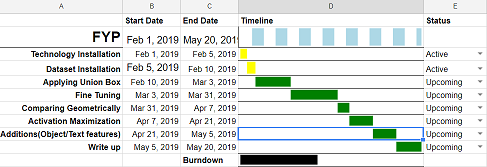
\includegraphics{Gantchart.png}}}
\end{center}
\caption{Gantt Chart} \label{f:pic}
\end{figure}

\section*{Acknowledgements.}
I would like to thank Dr Adrian Muscat for assisting me and guiding me through out this final year project .

\bibliographystyle{alpha}
\bibliography{refs}


\begin{thebibliography}{9}
\bibitem{ActivationMaximization1} 
Sebastian Lapuschkin, Alexander Binder, Gregoire Montavon, Klaus-Robert Muller and Wojciech Samek . 
\textit{Analyzing Classifiers Fisher Vectors and Deep Neural Networks}. 
Singapore University of Technology and Design, 2016.
 
\bibitem{ActivationMaximization2} 
Gregoire Montavona, Wojciech Samekb,Klaus-Robert Mullera. 
\textit{Methods for Interpreting and Understanding Deep Neural Networks}. 
 Technische Universita Berlin, Marchstr, 2017.

\bibitem{Spatial1} 
Yaohu iZhu and Shuqiang Jiang. 
\textit{Deep Structured Learning for Visual Relationship Detection}. 
 Chinese Academy of Sciences , 2017

\bibitem{ActivationMaximization3} 
Matthew D. Zeiler and Rob Fergus. 
\textit{Visualizing and Understanding Convolutional Networks}. 
 New York University, 2012.

\bibitem{Spatial2} 
 Anja Belz Computing and Adrian Muscat.
\textit{SpatialVOC2K A Multilingual Dataset of Images with Annotations and Features for Spatial Relations between Objects}. 
INSA Rouen Normandie 685 Avenue de l’Universite 76800 Saint-Etienne-du-Rouvray, France , 2017.

\bibitem{Spatial2} 
Arnau Ramisa , Josiah Wang , Ying Lu ,Emmanuel Dellandrea, Francesc Moreno-Noguer , Robert Gaizauskas.
\textit{Combining Geometric,Textual and Visual Features for Predicting Preposition Image Descriptions}. 
 University of Sheffield , 2015.


\end{thebibliography}

\end{document}
